\documentclass[protokol.tex]{subfiles}
\begin{document}
\begin{comment}
\begin{table}[H] \label{tab:podminky}
\centering
\setlength{\tabcolsep}{10pt}
\begin{tabular}{ccc}                                                    \toprule
Teplota                 &   Tlak                    &   Vlhkost     \\
$[\si{\degreeCelsius}]$ &   $[\si{\hecto\pascal}]$  &   [\% RH]     \\  \midrule
25,3                    &   984,5                   &   29,8        \\  \bottomrule
\end{tabular}
\caption{Podmínky měření}
\end{table}

\begin{figure}[H]
\centering
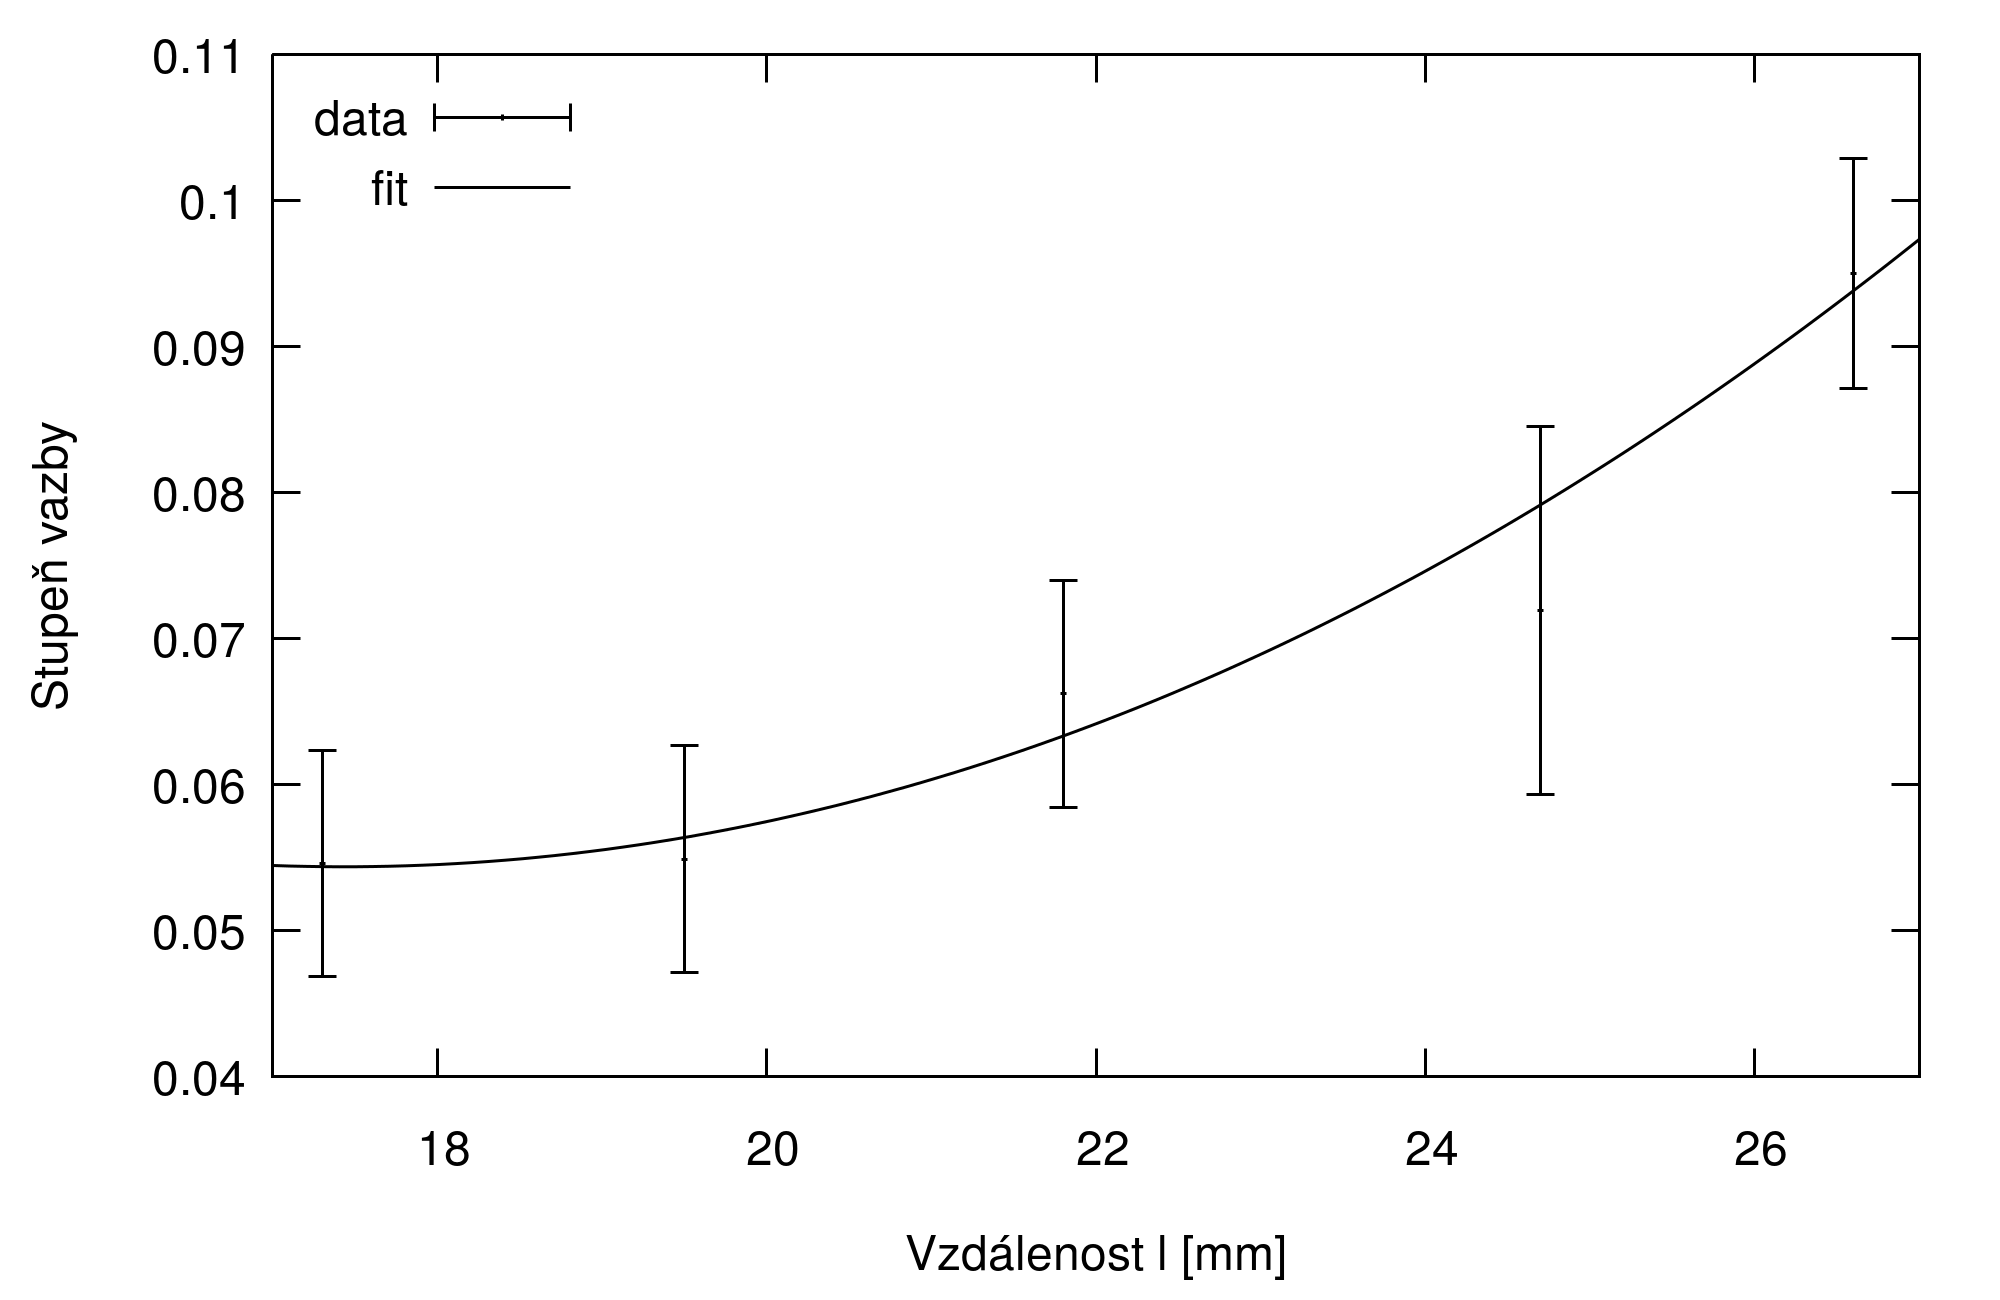
\includegraphics[resolution=350]{plot/graf}
\caption{Graf závislosti napětí na relativním prodloužení}
\end{figure}
\end{comment}
\begin{table}[H] \label{tab:podminky}
\centering
\setlength{\tabcolsep}{10pt}
\begin{tabular}{ccc}                                                    \toprule
Teplota                 &   Tlak                    &   Vlhkost     \\
$[\si{\degreeCelsius}]$ &   $[\si{\hecto\pascal}]$  &   [\% RH]     \\  \midrule
25,3                    &   984,5                   &   29,8        \\  \bottomrule
\end{tabular}
\caption{Podmínky měření}
\end{table}

\subsection*{Úkol 1}
Hodnota zobrazená na stupnici zrcátkem při základním zatížení drátu byla 
$$ n_0 = (147,0 \pm 0,5) \ \si{\milli\metre} $$

\newpage

Pomocí postupu popsaném v \cite{stud_text} se získaly hodnoty na svislé stupnici v závislosti na hmotnosti závaží, napínající drát. Hodnoty v následující tabulce mají chybu $\pm 0,5 \ \si{\milli\metre}$.
\begin{table}[H] \label{tab:drat_prodlouzeni}
\centering
\setlength{\tabcolsep}{15pt}
\begin{tabular}{cccc}                                                                                   \toprule
$ m [\si{\gram}]$   &   $n [\si{\milli\metre}]$ &   $ m [\si{\gram}]$   &   $n [\si{\milli\metre}]$ \\  \midrule
1,1                 &   144,8                   &   1,8                 &   129,0                   \\  
1,2                 &   142,3                   &   1,9                 &   126,8                   \\
1,3                 &   140,0                   &   2,0                 &   124,8                   \\
1,4                 &   137,8                   &   2,1                 &   122,5                   \\
1,5                 &   135,8                   &   2,2                 &   120,3                   \\
1,6                 &   133,3                   &   2,3                 &   118,0                   \\
1,7                 &   131,3                   &   2,4                 &   116,0                   \\  \bottomrule
\end{tabular}
\caption{Hodnota na stupnici v závislosti na hmotnosti závaží}
\end{table}

Poloměr kladky $r$ byl měřen posuvným měřidlem jako průměr, následně vydělený dvěma.
$$ r = (19,28 \pm 0,01) \ \si{\milli\metre} $$

Délka drátu od upevnění ke kladce $l_0$ byla měřena pásovým měřidlem, k naměřené hodnotě byla poté přičtena $\frac{1}{8}$ obvodu kladky.
$$ l_0 = (1156,1 \pm 1,2) \ \si{\milli\metre} $$

Délka $L$ od zrcátka ke stupnici byla ěřena pásovým měřidlem.
$$ L = (810 \pm 1) \ \si{\milli\metre} $$

Průměr drátu $d$ byl měřen na třech místech mikrometrem.
$$ d = (0,51 \pm 0,01) \ \si{\milli\metre} $$

Prodloužení drátu po přidání závaží s celkovou hmotností $1400 \si{\gram}$ spočítáme podle \eqref{eq:delta_l_2}:
$$ \Delta l = (0,369 \pm 0,008) \ \si{\milli\metre} $$

Modul pružnosti v tahu poté je z \eqref{eq:modul_dratu} 
$$ E = (2,1 \pm 0,1) \times \num{e11} \ \si{\pascal} $$

\newpage

\subsection*{Úkol 2}
Pomocí postupu popsaném v \cite{stud_text} jsme naměřili prohnutí $y_o$ ocelového trámku a $y_m$ trámku mosazného. Chyba hodnot v tabulce je $\pm 0,05 \si{\milli\metre}$.

\begin{table}[H] \label{tab:prohnuti}
\centering
\setlength{\tabcolsep}{10pt}
\begin{tabular}{cccc}                                                                   \toprule
$ m [\si{\gram}]$   &   $y_o [\si{\milli\metre}]$   &   $y_m [\si{\milli\metre}]$   \\  \midrule
10                  &   0,10                        &   0,18                        \\  
20                  &   0,20                        &   0,38                        \\  
30                  &   0,30                        &   0,53                        \\  
40                  &   0,40                        &   0,73                        \\  
50                  &   0,50                        &   0,90                        \\  
60                  &   0,60                        &   1,08                        \\  
70                  &   0,70                        &   1,28                        \\  
80                  &   0,80                        &   1,48                        \\  
90                  &   0,90                        &   1,63                        \\  
100                 &   1,00                        &   1,83                        \\  \bottomrule

\end{tabular}

\caption{Prohnutí trámku v závislosti na hmotnosti}
\end{table}

Vzdálenost mezi břity $l$ byla měřena pásovým měřidlem.
$$ l = (412 \pm 1) \ \si{\milli\metre} $$

Rozměry $a$ a $b$ trámků byly měřeny na třech místech mikrometrem.
$$ a_o = (11,98 \pm 0,02) \ \si{\milli\metre} $$
$$ b_o = (1,95  \pm 0,01) \ \si{\milli\metre} $$
$$ a_m = (11,84 \pm 0,03) \ \si{\milli\metre} $$
$$ b_m = (1,98  \pm 0,01) \ \si{\milli\metre} $$

Z \eqref{eq:modul_prohnuti} spočítáme
$$ E_o = (1,9 \pm 0,1) \times \num{e11} \si{\pascal} $$
$$ E_m = (1,02 \pm 0,03) \times \num{e11} \si{\pascal} $$

\newpage

\subsection*{Úkol 3}
Následující graf zachycuje závislost $\sigma$ na $\epsilon$ podle \eqref{eq:modul_dratu}. Lineární regrese byla provedena pomocí rovnice $y = Ex + b$.
\begin{figure}[H]
\centering
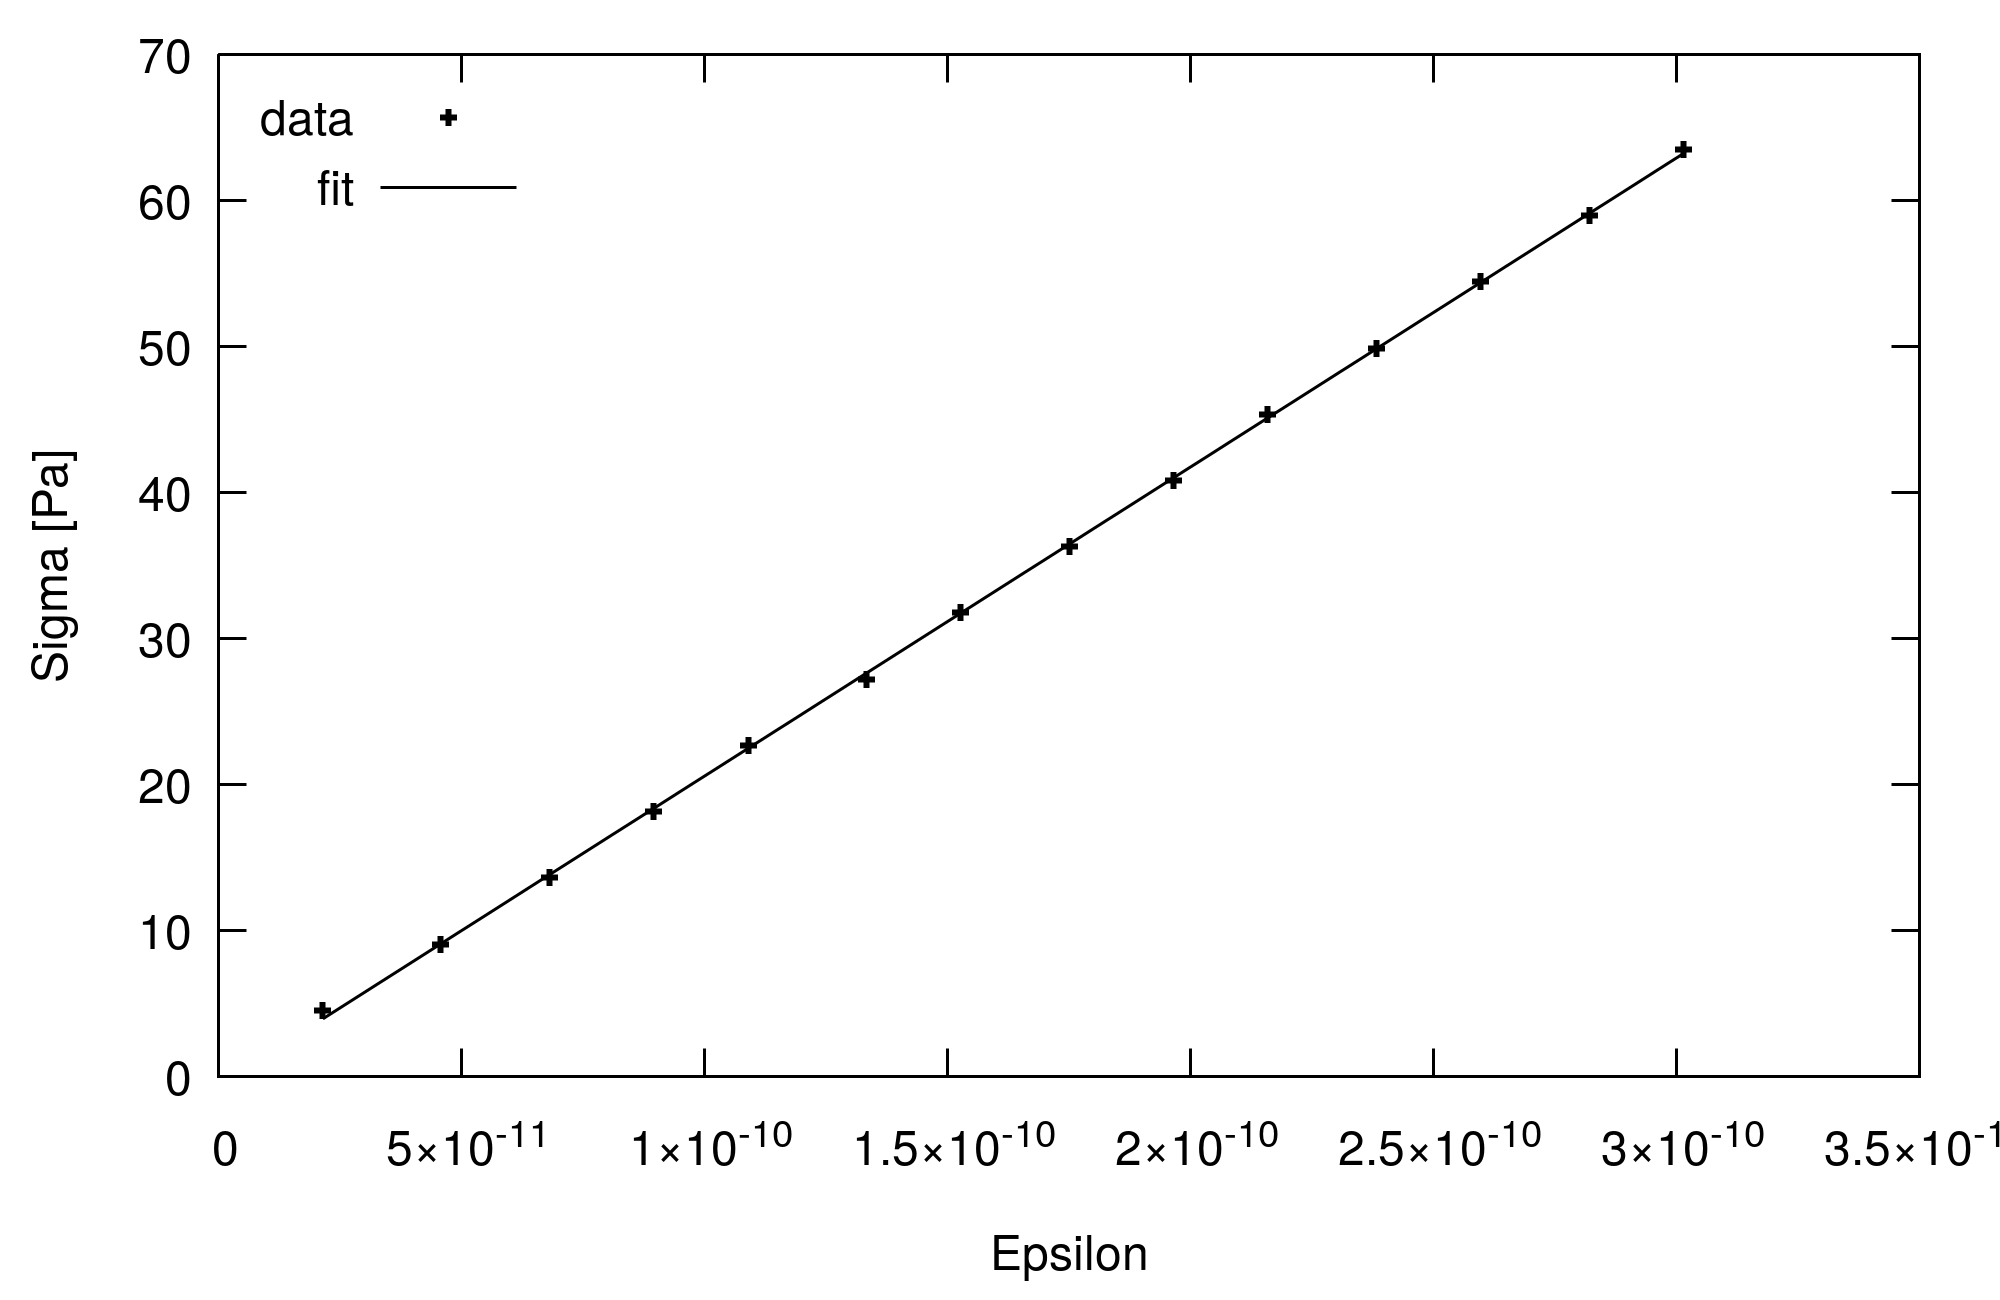
\includegraphics[resolution=350]{plot/drat}
\caption{Graf závislosti napětí na relativním prodloužení}
\end{figure}

$$ E = (2,1 \pm 0,1) \times \num{e11} \ \si{\pascal} $$
\end{document}
